\begin{center}
    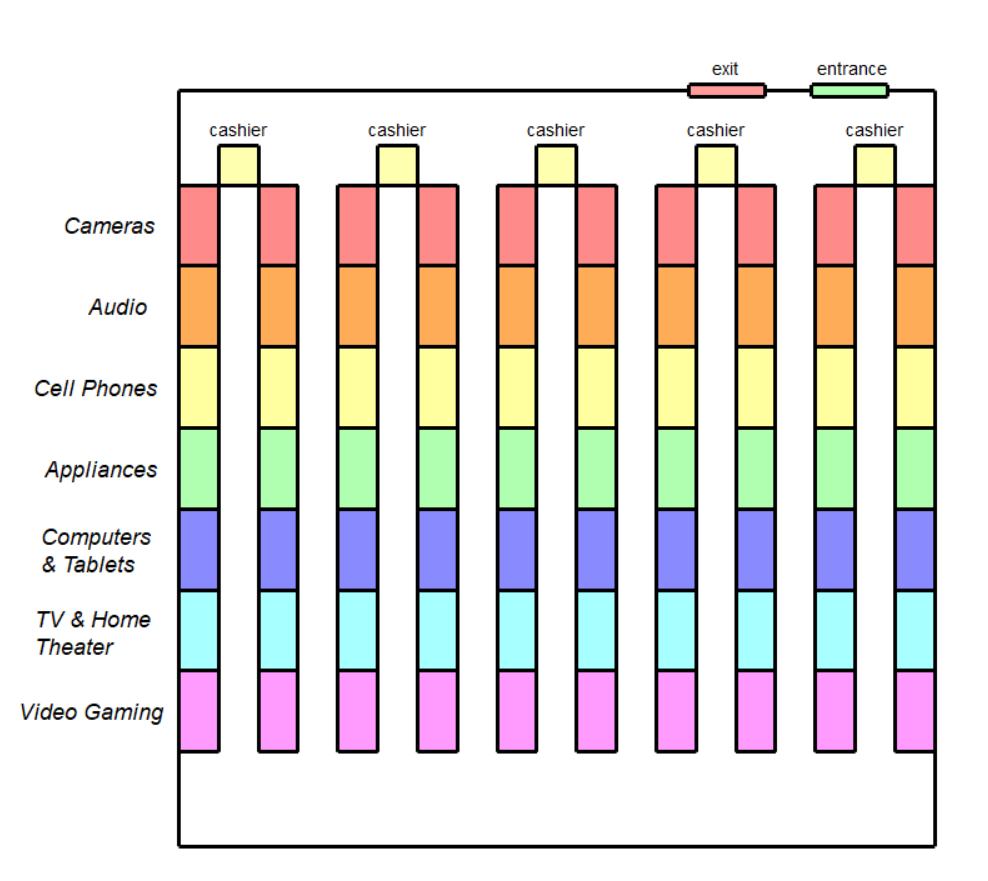
\includegraphics[width=\textwidth]{fig4.3.PNG}
\end{center}

First we define ProductID of each product by iterating over all the element in the given dataset and we let the first one be the product with ProductID = 0, and the next one having ProductID = 1 and so on.
\newline \par
Five shelves in above figure are organized identically following this given rule.
\newline
\par For every left shelf, we place product by this following sequence (from bottom to top)
\newline
42, 39, 33, 38, 35, 32, 45, 44, 18, 14, 13, 10, 12, 23, 20, 29, 28, 25, 27, 6, 7, 2, 1, 54, 55, 53, 64, 67, 69, 65, 60, 56, 62, 46, 48, 49, 85, 72, 76, 74, 78, 82, 80, 98, 92, 96, 95, 105, 99, 103, 104, 106, 114, 117, 116, 118, 111, 112, 86, 89, 87, 121, 122, 125, 126, 132, 130, 
\newline \par
For every right shelf, we place product by this following sequence (from bottom to top) \newline
41, 40, 34, 37, 36, 31, 43, 16, 17, 15, 9, 11, 21, 19, 22, 30, 24, 26, 5, 4, 8, 3, 0, 52, 51, 70, 63, 68, 66, 57, 59, 58, 61, 47, 50, 84, 75, 73, 71, 77, 81, 79, 83, 91, 97, 94, 93, 102, 101, 100, 108, 107, 119, 115, 120, 109, 110, 113, 88, 90, 124, 123, 129, 127, 128, 131, 133, 

\begin{center}
    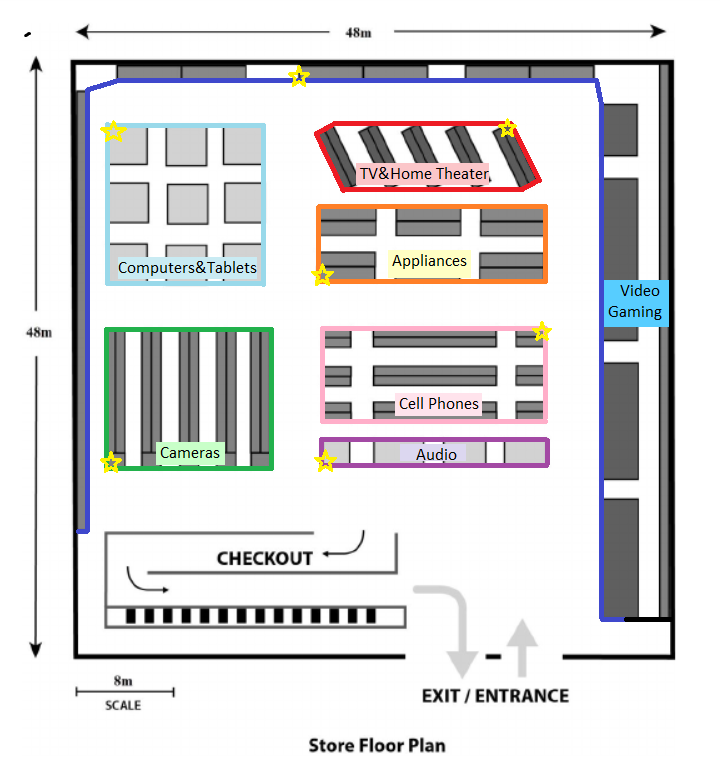
\includegraphics[width=\textwidth]{fig4.4.PNG}
\end{center}

legend - star indicates the most popular products in the department